% 2-3 page summary of the findings of the Backgrounds WG
\label{app:background}
%\noindent {\bf Chapter editors / working group conveners:}~Juliette Alimena, Martino Borsato, Zhen Liu, Sascha Mehlhase\\
% largely based on https://goo.gl/fw95iR

% -----------------------------------------------------------------------------------
\section{Introduction} % Sascha, all
% -----------------------------------------------------------------------------------

For many searches for LLPs, the main backgrounds do not stem from irreducible SM processes, but arise instead from \textit{external sources}. Indeed, there can even be backgrounds of instrumental and/or algorithmic nature. Often, LLP searches are designed to have a very small number of background events, sometimes even zero events, that pass the full selection criteria. This chapter gives an overview of common LLP search backgrounds and the means to estimate or control them.

% -----------------------------------------------------------------------------------
\section{Long-Lived Particles in the Standard Model} % Martino
\label{smbkg}
% -----------------------------------------------------------------------------------
Weak decays of SM particles can naturally give rise to displaced vertices at the boosts typically encountered at the LHC. Searches for LLP signatures at sufficiently low  LLP mass and lifetime suffer from large backgrounds due to displaced SM decays. One simple example is found in the search for long-lived dark photons  decaying to $\mu^+ \mu^-$ at LHCb~\cite{Aaij:2017rft}, which drastically loses sensitivity when the dark photon mass gets too close to the $K_{\rm S}\rightarrow\pi^+\pi^-$ invariant mass, despite the very low $\pi\rightarrow\mu$ misidentification rate.

Moreover, \textit{b}-hadrons can decay at displacements of a few mm and can be challenging to distinguish from LLPs with masses of a few tens of GeV that decay to a pair of jets. Requiring a large track multiplicity of the displaced vertex and performing a mass fit to the dijet invariant mass can help to significantly reduce the effect of this background (see, for example, Ref.~\cite{CMS:2014wda, Aaij:2017mic}). Backgrounds from heavy flavors are typically more abundant in the forward region, as arises, for example, if the signature under study is an LLP from the decay of a SM-like Higgs boson. However, the LHCb forward detector, which was designed to study these SM decays, is, in most cases, capable of rejecting heavy flavor backgrounds more effectively than can be done in ATLAS or CMS. Furthermore, displaced tracks from \textit{b}-mesons, which usually have impact parameters ($d0$) of less than 2 mm, can be rejected by using a larger criterion for the minimum track $d0$.

% -----------------------------------------------------------------------------------
\section{Real Particles Produced via Interactions with the Detector} % Martino, Sascha
% -----------------------------------------------------------------------------------

Particles produced in the $pp$ collision can interact with nuclei of the detector material, giving rise to displaced vertices, and can mimic LLP signals. Vertices from these interactions will be positioned in regions of the detector containing high densities of detector material and are therefore effectively vetoed by using detailed material maps.

The LHC detectors have developed tools internal to the collaborations to define a material volume to be vetoed. As the detector configurations changed slightly from Run 1 to Run 2, material maps have been determined separately for each data-taking period for both the ATLAS and CMS collaborations, using collision data. Maps can be found for ATLAS for Run 1 in Ref.~\cite{Aaboud:2016poq}, CMS for Run 1 in Ref.~\cite{CMS:2010nua}, ATLAS for Run 2 in Ref.~\cite{Aaboud:2017iio}, and CMS for Run 2 in Ref.~\cite{Sirunyan:2018icq}. Additionally, the Run 2 maps for both are shown here in Figures~\ref{fig:materialmapATLAS} and \ref{fig:materialmapCMS} for ATLAS and CMS, respectively.
%
\begin{figure}[t]
  \centering
  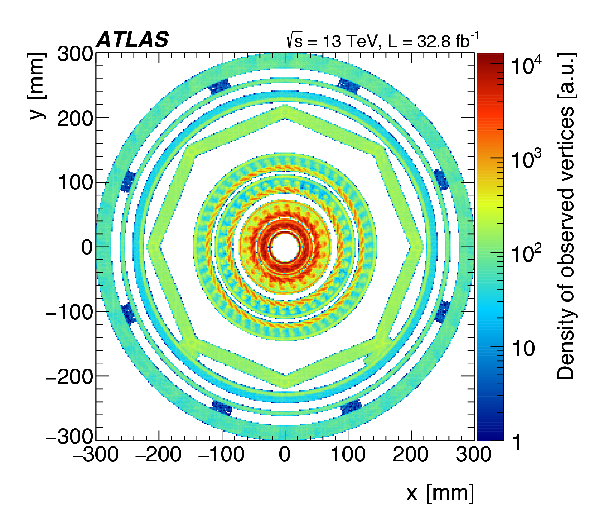
\includegraphics[width=0.8\textwidth]{figures/atlasmaterial.pdf}
  \caption{An example of a material map from ATLAS~\cite{Aaboud:2017iio}.
  }
  \label{fig:materialmapATLAS}
\end{figure}

%
\begin{figure}[t]
  \centering
   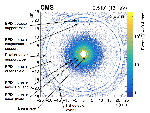
\includegraphics[width=0.9\textwidth]{figures/cmsmaterial.pdf}
  \caption{An example of a material map from CMS~\cite{Sirunyan:2018icq}.
  }
  \label{fig:materialmapCMS}
\end{figure}

LHCb recently developed a precise material map of the VErtex LOcator (VELO) using beam-gas collisions~\cite{Alexander:2018png}, shown in Figure~\ref{fig:lhcbmaterialmap}. Beam-gas collisions can be distinguished from long-lived heavy flavor backgrounds and their utilization allows the map to cover precisely the whole VELO geometry, not only the region close to the interaction point. This map was used to veto photon conversions to di-muons, which is the main background affecting displaced dark-photon searches at low mass~\cite{Aaij:2017rft}. In analyses, this material map, together with properties of a reconstructed secondary vertex and its constituent tracks, is used to construct a $p$-value that is assigned to the hypothesis that the secondary vertex originates from a material interaction. As a rule of thumb, LHCb material interaction background is dominant for vertices at a distance from the beam axis larger than 6~mm (where the VELO material begins). Below 6~mm the background is dominated by heavy flavor decays~\cite{Ilten:2016tkc}.

\begin{figure}[t]
  \centering
  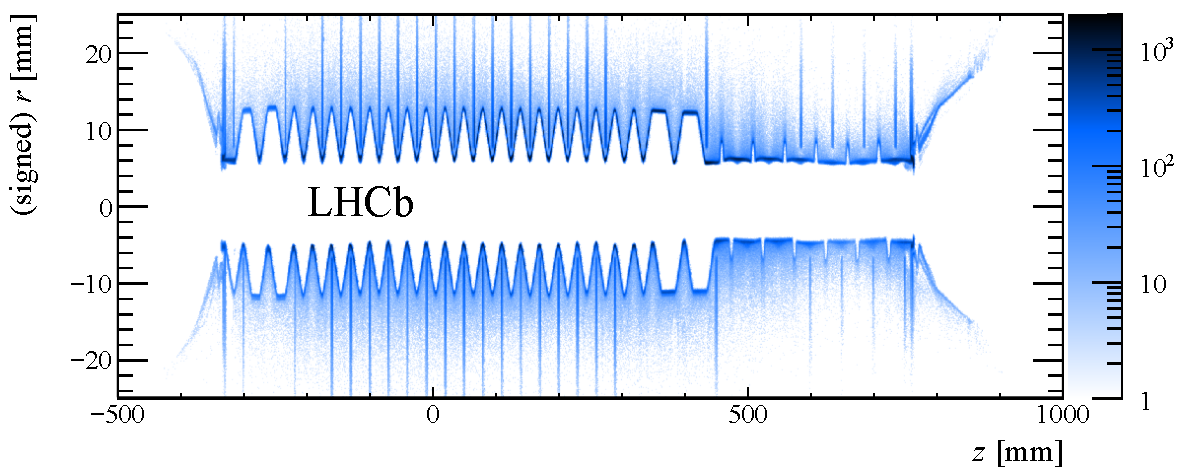
\includegraphics[width=\textwidth]{figures/lhcbmaterial.pdf}
  \caption{Reconstructed secondary vertices in the LHCb VELO from beam-gas collisions in the $zr$ plane integrated over $\phi$. These vertices are used to build the material map~\cite{Alexander:2018png} to veto backgrounds from material interactions.
  }
  \label{fig:lhcbmaterialmap}
\end{figure}

Because accurate material maps are essential to performing fully reliable sensitivity studies to signatures with displaced vertices, making them publicly available to the broader LLP community is of the highest priority. The availability of such tools in fast parametric simulations such as Delphes~\cite{deFavereau:2013fsa} would be very useful to reinterpret LLP search results. In Section~\ref{sec:ch5-displacedVertexReconstruction}, an example of a reinterpretation of an LLP search is presented, where a rough material veto was performed because these material maps were not publicly available, highlighting the shortcomings of such approaches in the absence of accurate material maps and emphasizing the benefits of making them available.
%{\bf \textcolor{red}{JB: Do you mean that these maps ``were not'' available at the time the reinterpretation was performed?  Otherwise the implication is that the maps are presented here for the first time.}}

%ATLAS 7 TeV \cite{Aaboud:2016poq} (QUESTION: is it valid for Run 2?)
%CMS 7 TeV \cite{CMS:2010nua}
%CMS 13 TeV \cite{CMS-DP-2016-073,CMSmaterial} (there is no paper, am I right?) JA: We have a public detector performance note (CMS-DP-2016-073) and a newer public twiki than the original one you cited (I updated the reference). The the paper is about to enter CWR, so not public yet.

High-energy collision muons originating mainly from $W$ decays and creating secondary interactions in the tracker, calorimeters or muon system can be an additional source for displaced vertices mimicking LLP signals. This mostly minor background arises as vetoing these displaced vertices is based on a not 100\% efficient detection of the high-\pt track in the tracker.

Another important background, mainly for analyses targeting the reconstruction of decay vertices of long-lived particles reaching the muon systems, is hadronic or electromagnetic showers not contained in the calorimeter volume, so-called punch-through jets~\cite{Aad:2015uaa}. These punch-through jets occur especially in regions of reduced total interaction length in the calorimeters (e.g., transition regions between the barrel and the end-caps) and can be suppressed by either rejecting these $|\eta|$ regions or requiring a minimal number of hits in the muon system and isolating the displaced vertex from calorimeter jets as well as high-energy tracks and significant track activity in the inner tracking system. In order to not reject true vertices from displaced decays that occur near the end of the calorimeters, the calorimeter-jets veto should only consider jets with a minimum total energy deposit and, e.g., a minimum electromagnetic fraction of the total energy. The track isolation requirement aims at regions with a poor calorimeter measurement (again, transition regions in the calorimeters), where a single high-energy track or the sum of the track activity in a small cone around the displaced vertex could indicate a (punch-through) jet. On the other hand, punch-through jets, given their similarity to signal signatures, can also be used to evaluate systematic uncertainties due to imperfect modeling in the muon-system simulation.

% https://arxiv.org/abs/1504.03634 (used that for cite above)
% https://cds.cern.ch/record/2256102 (ATLAS)
% https://arxiv.org/abs/1703.09665
% https://cds.cern.ch/record/2636535 (ATLAS, to come out soonish; would rather use that as citation above)

% -----------------------------------------------------------------------------------
\section{Real Particles Originating from Outside the Detector} % Juliette
% -----------------------------------------------------------------------------------

There are several types of real particles generated outside the detector that could be sources of background in an LLP search.

% -----------------------------------------------------------------------------------
\subsection{Cosmic muons} % Juliette
% -----------------------------------------------------------------------------------

Cosmic rays from the atmosphere can enter the detector as cosmic-ray muons. These cosmic-ray muons can be reconstructed as displaced muons in the muon system or as displaced jets in the calorimeters. If cosmic-ray muons are reconstructed in the muon systems, they will typically appear as two back-to-back muons with $\phi$ values near $\pm\pi/2$. The rate of cosmic muons in the detector is about 500~Hz at L1, but depending on the HLT path and the offline selection used, the rate of cosmic-ray muons entering a given LLP analysis is generally much less.

Cosmic-ray muons are typically an important background source to consider for displaced signatures, especially those with large displacements~\cite{Khachatryan:2015jha, Chatrchyan:2012dxa, Khachatryan:2010uf, Aad:2012zn,Aad:2013gva}. Cosmic-ray muons are generally only an issue for LLP analyses in CMS and ATLAS since LHCb has coverage only in the forward direction.

For many analyses, cosmic-ray muons can be rejected with a simple veto on back-to-back dimuons. However, in some LLP analyses, this veto is not optimal for the signal acceptance or it is insufficient to suppress cosmic-ray backgrounds. Another often-used way to minimize the contribution from cosmic-ray muons is requiring high-momentum muons and/or high-energy jets, since cosmic-ray muons have a rapidly falling $p_{T}$ spectrum. In addition, if a search primarily looks for inner-tracker or calorimeter objects, cosmic-ray-muon events can be rejected by requiring little muon system activity~\cite{Khachatryan:2015jha, Chatrchyan:2012dxa, Khachatryan:2010uf}.

If the cosmic-ray muon background is significant for an analysis, it can be estimated using data from dedicated cosmic data-taking runs or from empty bunches in $pp$ collision runs~\cite{Khachatryan:2015jha, Chatrchyan:2012dxa, Khachatryan:2010uf}. Cosmic ray muon simulations can be made, but in many LLP analyses, a data-driven approach is favoured if the simulation modeling is found to be insufficent. Timing information in the calorimeters or the muon systems can be used to discriminate the signal from cosmic-ray muons, sometimes in conjunction with impact parameter variables.

% -----------------------------------------------------------------------------------
\subsection{Beam halo} % Juliette
% -----------------------------------------------------------------------------------

Another type of real particle generated outside the detector that could be a significant source of background for LLP searches is beam halo. Beam halo is produced when protons from the LHC beam scatter off the LHC collimators and produce debris, which can appear in the detector. Beam halo can create energy deposits in the calorimeters or hits in the muon system, both of which would be largely in the beam direction. These energy deposits or muon system hits would appear earlier than if they had been made from particles coming from the collision (see Figure~\ref{fig:beamHaloSketch}). Beam halo is usually not modelled in MC simulation, since it is highly dependent on the beam parameters.

\begin{figure}[t]
  \centering
  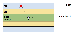
\includegraphics[width=\textwidth]{figures/beamHaloSketch.pdf}
  \caption{A sketch illustrating the timing differences due to the shorter, more direct path to the calorimeter cells between a beam-halo muon and a particle originating from the collision. The beam-halo muon is detected earlier than the particle from the collision.}
  \label{fig:beamHaloSketch}
  % sketched by Sascha in https://goo.gl/fw95iR
\end{figure}

Beam halo is most relevant for searches for displaced signatures without tracks in the inner tracker and for searches for decays in non-collision bunches (e.g., from stopped particles)~\cite{Khachatryan:2015jha, Chatrchyan:2012dxa, Khachatryan:2010uf}, which are described in Section~\ref{subsec:funnytracks}.

The contribution from beam halo can often be reduced by requiring high-momentum or high-energy reconstructed objects. One can also decrease the number of beam halo events by requiring central objects or vetoing forward muon system activity, since beam halo is usually in the very forward direction~\cite{Khachatryan:2015jha, Chatrchyan:2012dxa, Khachatryan:2010uf}. For inner tracker-based signatures, events from beam halo are rejected by requiring a minimum number of early hits; in this way beam halo is rejected due to its anomalous timing.

Beam halo background can be estimated using data control regions near $\phi=0$ and $\pi$. One could also identify cells with a low number of (or zero) tracks that are assigned an early time. %where are the cells - calo? Do we have an example banana plot to show?

% -----------------------------------------------------------------------------------
\subsection{Cavern radiation} % Juliette/Sascha
% -----------------------------------------------------------------------------------

Diffuse backgrounds can also arise from proton--proton collisions filling the LHC caverns, consisting mostly of neutral, low-energy, and long-lived SM particles (i.e., neutrons and photons), leading to an overall increase in occupancy, especially in the muon systems. This so-called ``cavern background'' or ``cavern radiation'' can constitute a significant background in a LLP search. As simulations are resource-intensive, it is usually not at all modelled in MC simulation samples.

Cavern radiation is most relevant for searches looking in non-collision data, that is, stopped-particle searches, and for searches using muon system information to form tracks and vertices. It can be estimated from data by collecting events triggered by random triggers when there are no collisions, as was done in Ref.~\cite{Aad:2013gva}.~\footnote{Note that these triggers are unlike those used to collect the search data for stopped-particle searches, which instead select events with physics objects during empty bunch crossings.} Cavern radiation can also be estimated by overlaying a cavern radiation simulation with minimum-bias events from data.

% some in depth studies of radiation background in ATLAS http://cdsweb.cern.ch/record/814823/files/gen-2005-001.pdf % Sascha
% RPC cavern background in ATLAS http://cdsweb.cern.ch/record/1457509/files/ATL-MUON-PROC-2012-005.pdf % Sascha
% MC cavern background in ATLAS http://inspirehep.net/record/1409861/files/507_510.pdf % Sascha
% MS studies in ATLAS https://indico.cern.ch/event/279530/contributions/634992/attachments/511921/706530/ATLAS-MS-CavernBackground.pdf % Sascha
% Geant4 studies in ATLAS http://atlas.web.cern.ch/Atlas/GROUPS/PHYSICS/MUON/PublicPlots/2014/ATL-COM-MUON-2014-018/ % Sascha

% -----------------------------------------------------------------------------------
\section{Fake-Particle Signatures} % Juliette
% -----------------------------------------------------------------------------------

Another type of background for LLP searches is that from signatures that mimic real particles in the detector, but are in fact fake. Fake particles can originate from spurious detector noise. Noise appears differently for each detector, but in general, it is characterized by a single and concentrated energy deposit or hit that does not correspond in time or space to any other energy deposits or hits in the detector. Noise is usually difficult to model with MC simulation.
%SM - general question: do we wanna use personal terms like "we do ..." or avoid it?
%JA - Yeah, maybe not, but I think this is a style question that would be good to have consistent across all sections of the white paper, so I suggest we leave it for when the sections get combined again.

Calorimeter detector noise is most relevant for searches looking in non-collision bunches and low-energy collisions~\cite{Khachatryan:2015jha, Chatrchyan:2012dxa, Khachatryan:2010uf}. Muon system noise is most relevant for searches that are also highly affected by cosmic-ray muons.

Calorimeter noise can be rejected by vetoing single and concentrated energy deposits~\cite{Khachatryan:2015jha, Chatrchyan:2012dxa, Khachatryan:2010uf}. Muon system noise can be rejected by requiring high-quality muon tracks.

Noise in both the calorimeters and the muon systems could be estimated by looking at dedicated cosmic data-taking runs and then applying some selection criteria to reject cosmic-ray muons. The remaining events would most likely be noise.

% -----------------------------------------------------------------------------------
\section{Algorithmically Induced Fakes} % Sascha
% -----------------------------------------------------------------------------------

For searches that aim to reconstruct the decay vertex of an LLP, and especially for long-lived particles decaying in the proximity of the interaction region, algorithmically induced fakes and/or instrumental backgrounds can be of importance. Algorithmic fakes can still be a significant background to LLP searches, even if a given detector is noise-free.

% -----------------------------------------------------------------------------------
\subsection{Random/Merged Vertices} % Sascha
% -----------------------------------------------------------------------------------

This type of background, illustrated in Figure~\ref{fig:mergedvertices}, is especially important in the environment close to the interaction region that experiences a high track density, and arises from two main sources. First, two or more individual tracks can cross each other and can be reconstructed as a displaced vertex. Second, two close-by, low-mass vertices can be reconstructed as one high-mass displaced vertex; such a final merging/cleaning step is often part of vertexing algorithms to reduce fakes in standard vertexing.

\begin{figure}[h]
  \centering
  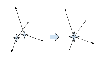
\includegraphics[width=0.7\textwidth]{figures/mergedvertices.pdf}
  \caption{Illustration of two close-by, low-mass vertices being reconstructed as one high-mass vertex.}
  \label{fig:mergedvertices}
  % sketched by Sascha in https://goo.gl/fw95iR
\end{figure}

The former source is mostly suppressed by requirements originally targeting the removal of meta-stable SM particles:~a minimum transverse impact parameter, $|d_0|$, for tracks and a minimum distance between the primary vertex and a given displaced vertex.

The latter source is harder to suppress, though can be estimated by randomly merging vertices from distinct events. By studying the number of reconstructed ``merged'' high-mass vertices as a function of distance between the two low-multiplicity low-mass vertices that were ``merged'' --- both with vertices from the same event, as well as from different events and scaling them accordingly --- an estimate for this background can be derived. This method has been successfully used in the ATLAS search for displaced vertices~\cite{Aaboud:2017iio} and the ATLAS multitrack analysis~\cite{Aad:2015rba}.

% -----------------------------------------------------------------------------------
\subsection{Randomly Crossing Tracks} % Sascha
% -----------------------------------------------------------------------------------

A background that is typically more relevant than merged vertices is the background stemming from low-mass displaced vertices crossed by unrelated tracks, resulting in the reconstruction of a high-mass vertex, as illustrated in Figure~\ref{fig:randomcrossing}. The mass of the reconstructed displaced vertex is especially increased when the random track crosses the vertex in a direction that is perpendicular to the distance vector pointing from the primary vertex to the displaced one.

\begin{figure}[h]
  \centering
  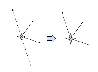
\includegraphics[width=0.7\textwidth]{figures/randomcrossing.pdf}
  \caption{Illustration of a low-mass vertex crossed by an unrelated track and being reconstructed as a high-mass vertex instead.}
  \label{fig:randomcrossing}
  % sketched by Sascha in https://goo.gl/fw95iR
\end{figure}

As demonstrated in detail in Ref.~\cite{Aaboud:2017iio,Aad:2015rba}, this background can be estimated by constructing vertices ($n$-track) from lower-multiplicity ones ($n-1$-track) by adding pseudo-tracks, drawn randomly from data-driven track templates derived for various radial detector regions. The normalization of the prediction is performed by comparing the $n-1$-track-based constructed vertices with the actual n-track vertices in all radial detector regions. One potential method for suppressing such backgrounds is to veto vertices where removing one track substantially decreases the mass of tracks associated with the vertex.

% -----------------------------------------------------------------------------------
\section{Summary} % all
% -----------------------------------------------------------------------------------

LLP searches often have very low backgrounds, as opposed to searches for prompt particles. This makes LLP searches highly sensitive to signals of new physics.

There are, however, a few common sources of background that arise in different LLP searches:~other, known, long-lived particles such as \textit{b}-hadrons; real particles produced in the detector, such as particles produced in collisions that interact with the nuclei of the detector material; real particles produced outside the detector, such as cosmic muons or beam halo; fake particles, such as detector noise; and algorithmically induced fakes, such as two tracks that cross and are reconstructed as a displaced vertex, as described above. These backgrounds are generally atypical, difficult to model in simulation, and challenging to estimate. Thus, the possible appearance of unexpected background sources should be taken into account in any new LLP search, and the development of novel techniques and methods to estimate them is encouraged.
% We recommend that analyses provide separate background estimates for each source of background considered, rather than providing an estimate for one or more groups of different background sources.
